\documentclass[../main.tex]{subfiles}
\graphicspath{{\subfix{../images/}}, {\subfix{../}}}

\begin{document}

\chapter{Ginzburg-Landau theory of superconductivity}

\section{Coherence length and penetration depth in strongly correlated superconductors}

From~\cite{wittBypassingLatticeBCSBEC2024}.

In most materials: Cooper pairs do not carry finite center-of-mass momentum.
In presence of e.g.\ external fields or magnetism: SC states with FMP might arise.

Theory/procedure in the paper: enforce FMP states via constraints on pair-center-of-mass momentum \(\vb{q}\), access characteristic lenght scales \(\xi_0, \lambda_L\) through analysis of the momentum and temperature-dependent OP\@.
Constrain for FF-type pairing:
\begin{equation}
    \psi_{\vb{q}} (\vb{r}) = \vert \psi_{\vb{q}} \vert e^{\iu \vb{q} \vb{r}}
\end{equation}


\section{Phase transitions and broken symmetry}

Following~\cite[ch. 11]{colemanIntroductionManyBodyPhysics2015}.

\subsection{Order parameter concept}

Landau theory: phase transitions (e.g.\ iron becomes magnetic, water freezes, superfluidity/superconductivity) are associated with the development of an order parameter when the temperature drops below the transition temperature \(T_C\).
\begin{equation}
    \vert \psi \vert =
    \begin{cases}
        0\;,\; T > T_C \\
        \vert \psi_0 \vert > 0 \;,\; T < T_C
    \end{cases}
\end{equation}
Landau theory does not need microscopic expression for order parameter, it provides corse-grained description of the properties of matter.
The order parameter description is good at length scales above \(\xi_0\), the coherence length (e.g.\ size of Cooper pairs for SC).

\subsection{Landau theory}

Basic idea of Landau theory: write free energy as function \(F[\psi]\) of the order parameter.
Region of small \(\psi\), expand free energy of many-body system as simple polynomial:
\begin{equation}
    f_{L} = \frac{1}{V} F[\psi] = \frac{r}{2} \psi^2 + \frac{u}{4} \psi^4
\end{equation}
Provided \(r\) and \(u\) are greater that \(0\): minimum of \(f_L [\psi])\) lies at \(\psi = 0\).
Landau theory assumes: at phase transition temperature \(r\) changes sign, so:
\begin{equation}
    r = a(T - T_C)
\end{equation}
Minimum of free energy occurs for:
\begin{equation}
	\psi = \begin{cases}
		0 \\
		\pm \sqrt{\frac{a (T_C - T)}{u} }
	\end{cases}
\end{equation}

Two minima for free energy function for \(T < T_C\).
With this, we can extract \(T_C\) from the knowledge of the dependence of \(\vert \psi \vert^2\) on \(T\) via a linear fit.
This is only valid for an area near \(T_C\) (where Landau theory holds), but can be used to get \(T_C\) from microscopic theories.

\todo{Could put a bit more into here about second order phase transition}

Going from a one to a \(n\)-component order parameters, OP acquires directions and magnitude.
Particularly important example: complex or two component order parameter in superfluids and superconductors:
\begin{equation}
    \psi = \psi_1 + \iu \psi_2 = \vert \psi \vert e^{\iu \phi}
\end{equation}
The Landau free energy takes the form:
\begin{equation}
    f[\psi] = r(\psi^* \psi) + \frac{u}{2} (\psi^* \psi)^2
\end{equation}
As before:
\begin{equation}
    r = a(T - T_C)
\end{equation}

Figure~\ref{fig:Landau free energy mexican hat potential} shows the Landau free energy as function of \(\psi\).

\begin{figure}[t]
    \centering
    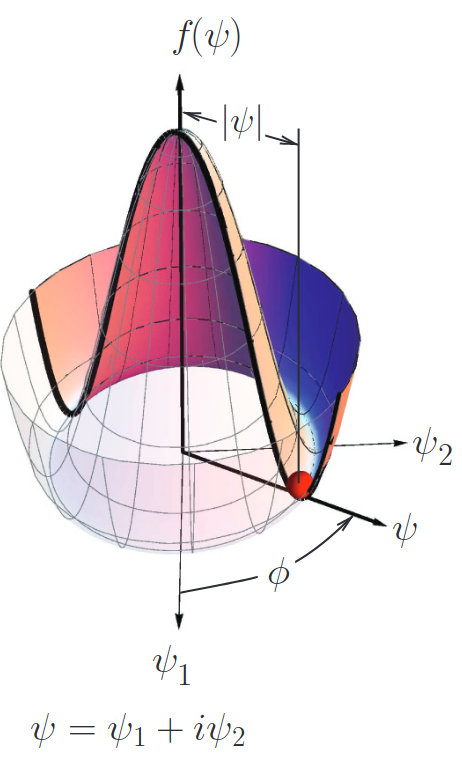
\includegraphics[width=0.3\textwidth]{images/landau free energy mexican hat}
    \caption{Mexican hat potential}
    \label{fig:Landau free energy mexican hat potential}
\end{figure}

Rotational symmetry, because free energy is independent of the global phase of the OP:
\begin{equation}
    f [\psi] = f [e^{\iu a } \psi]
\end{equation}
In this `Mexican hat' potential: order parameter can be rotated continuously from one broken-symmetry state to another.
If we want the phase to be rigid, we need to introduce an
There is a topological argument for the fact that the phase is rigid.
This leads to Ginzburg-Landau theory.
Will see later: well-defined phase is associated with persistent currents or superflow.

\subsection{Ginzburg-Landau theory I: Ising order}

Landau theory: energy cost of a uniform order parameter, more general theory needs to account for inhomogenous order parameters, in which the amplitude varies or direction of order parameter is twisted -> GL theory.
First: one-component, `Ising' order parameter.
GL introduces additional energy \(\delta f \propto \vert \Delta \psi \vert^2\), \(f_{GL} [\psi, \Delta \psi] = \frac{s}{2} \vert \Delta \psi \vert^2 + f_L [\psi(s)]\), or in full:
\begin{equation}
    f_{GL} [\psi, \Delta \psi, h] = \frac{s}{2} (\Delta \psi)^2 + \frac{r}{2} \psi^2 + \frac{u}{4} \psi^4 - h \psi
\end{equation}
\todo{What is the \(h\) here?}
GL theory is only valid near critical point, where OP is small enough to permit leading-order expansion.
Dimensional analysis shows: \(\frac{c}{r} = L^2\) \todo{What is c?} has dimension of length squared.
Length scale introduced by

\todo{length scale/correlation length}

\subsection{Ginzburg-Landau theory II: complex order and superflow}

Now: G-L theory of complex or two-component order parameters, so superfluids and superconductors.
Heart of discussion: emergence of a `macroscopic wavefunction', where the microscopic field operators \(\hat{\psi(x)}\) acquire an expectation value:
\todo{What exactly are field operators again?}
\begin{equation}
    \braket{\psi (x)} = \psi (x) = \vert \psi (x) \vert e^{\iu \theta(x)}
\end{equation}
Magnitude determines density of particles in the superfluid:
\todo{More info on that? Does that come later in chapter?}
\begin{equation}
    \vert \psi(x) \vert^2 = n_s (x)
\end{equation}
Twist/gradient of phase determines superfluid velocity:
\begin{equation}
    \vb{v}_s (x) = \frac{\hbar}{m} \Delta \phi (x)
\end{equation}
We will derive this later in the chapter.
Counterintuitive from quantum mechanics: GL suggested that \(\Phi(x)\) is a macroscopic manifestation of a macroscopic number of particles condensed into precisely the same quantum state.
Emergent phenomenon, collective properties of mater not a-priori self-evident from microscopic physics.

GL free energy density for superfluid (with one added term in comparison to Landau energy):
\begin{equation}
    f_{GL} [\psi, \Delta \psi] = \frac{\hbar^2}{2m} \vert \Delta \psi \vert^2 + r \vert \psi \vert^2 + \frac{u}{2} \vert \psi \vert^4
\end{equation}
Interpreted as energy density of a condensate of bosons in which the field operator behaves as a complex order parameter.
\todo{energy density of bosonic field? -> for comparison!}
Gives interpretation of gradient term as kinetic energy:
\begin{equation}
    s \vert \Delta \psi \vert^2 = \frac{\hbar^2}{2m} \braket{\Delta \hat{\psi}^{\dagger} \Delta \hat{\psi}} \implies s = \frac{\hbar^2}{2m}
\end{equation}
As in Ising order: correlation length/GL-coherence length governs characteristic range of amplitude fluctuations of the order parameter:
\begin{equation}
    \xi = \sqrt{\frac{s}{\vert r \vert}} = \sqrt{\frac{\hbar^2}{2m \vert r \vert}} = \xi_0 (1 - \frac{T}{T_C})^{-\frac{1}{2}}
\end{equation}
\todo{Compare with Ising order, especially dependence on \(T\)}
where \(\xi_0 = \xi(T=0) = \sqrt{\frac{\hbar^2}{2 m a T_C}}\) is the coherence length.
Beyond this length: only phase fluctuations survive.
\todo{Compare with Ising order. Is that derived or postulated?}
Freeze out fluctuations in amplitude (no \(x\)-dependence in amplitude) \(\psi(x) = \sqrt{n_s} e^{\iu \phi(x)}\), then \(\Delta \psi = \iu \Delta \phi \psi\) and \(\vert \Delta \psi \vert^2 = n_s (\Delta \phi)^2\), dependency of kinetic energy on the phase twist is (bringing it into the form \(\frac{m}{2} v^2\)):
\begin{equation}
    \frac{\hbar^2 n_s}{2m} (\Delta \phi)^2 = \frac{m n_s}{2} (\frac{\hbar}{m} \Delta \phi)^2
\end{equation}
So twist of phase results in increase in kinetic energy, associated with a superfluid velocity:
\begin{equation}
    \vb{v}_s = \frac{\hbar}{m} \Delta \phi
\end{equation}

For interpretation of superfluid states: coherent states.
These are eigenstates of the field operator
\begin{equation}
	\hat{\psi}(x) \ket{\psi} = \psi (x) \ket{\psi} 
\end{equation}
and don't have a definite particle number.
Importantly, this small uncertainty in particle number enables a high degree of precision in phase (which is the property of a condensate).

Phase rigidity and superflow: in GL theory, energy is sensitive to a twist of the phase.
Substitute \(\psi = \vert \psi \vert e^{\iu \phi}\) into GL free energy, gradient term is:
\begin{equation}
    \Delta \psi = (\Delta \vert \psi \vert + \iu \Delta \phi \vert \psi \vert) e^{\iu \phi}
\end{equation}
So:
\begin{equation}
	f_{GL}  = \frac{\hbar}{2m} \vert \psi \vert^2 (\Delta \phi)^2 + \left[ \frac{\hbar}{2m} (\Delta \vert \psi \vert)^2 + r \vert \psi \vert^2 + \frac{u}{2} \vert \psi \vert^4 \right]
\end{equation}
The second term resembles GL functional for an Ising order parameter, describes energy cost of variations in the magnitude of the order parameter.

\todo{Here: particle-current operator, especially for coherent state, connection with phase twist}

\end{document}